\begin{wrapfigure}{L}{0.5\textwidth}
	\vspace{-10pt}
	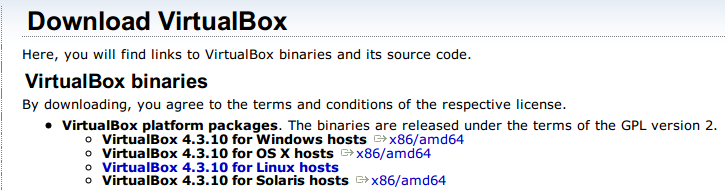
\includegraphics[width=\linewidth]{images/virtualbox_download.png}
\end{wrapfigure}

Alternatywnym sposobem wypróbowania Ubuntu bez instalowania go bezpośrednio na komputerze jest wykorzystanie maszyny wirtualnej. Specjalne oprogramowanie umożliwia uruchomienie systemu operacyjnego, zwanego ,,gościem'', jako programu działającego wewnątrz drugiego systemu, zwanego ,,gospodarzem''. Wiąże się to oczywiście z dużym zapotrzebowaniem na moc obliczeniową procesora oraz pamięć operacyjną. Jeżeli masz przynajmniej 2 gigabajty RAM-u, a twój procesor jest nie starszy niż 5 lat (wtedy jest szansa, że będzie zapewniał akcelerację sprzętową dla wirtualizacji), to możesz w ten sposób wypróbować Ubuntu.

\begin{wrapfigure}[11]{r}{0.5\textwidth}
	\vspace{-10pt}
	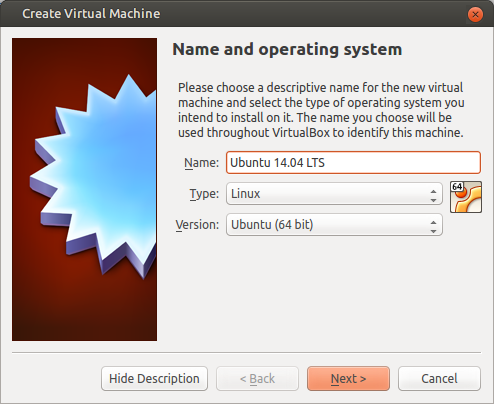
\includegraphics[width=\linewidth]{images/virtualbox_wizard1.png}
\end{wrapfigure}

Jedną z najpopularniejszych maszyn wirtualnych jest VirtualBox. Otwórz stronę \href{https://www.virtualbox.org/wiki/Downloads}{virtualbox.org/download} i pobierz instalator VirtualBoksa dla swojego systemu. Zainstaluj, a następnie uruchom program VirtualBox. Podczas pierwszego uruchomienia program zapyta cię, czy pobrać i zainstalować dodatkowe rozszerzenia od Oracle. Zgódź się na to.

W oknie głównym programu VirtualBox kliknij przycisk \textcolor{ubuntu_orange}{New}, aby uruchomić kreator maszyny wirtualnej.

\begin{itemize}
\item \textcolor{ubuntu_orange}{Name} --- nazwa maszyny wirtualnej. Może to być cokolwiek.
\item \textcolor{ubuntu_orange}{Type} --- typ systemu. Ustaw na \textcolor{ubuntu_orange}{Linux}.
\item \textcolor{ubuntu_orange}{Version} --- wersja systemu. Ustaw na \textcolor{ubuntu_orange}{Ubuntu (64 bit)}.\\
Uwaga: Architektura wybranego systemu (32/64 bit) musi odpowiadać pobranemu obrazowi instalatora Ubuntu. Dodatkowo należy pamiętać, że w komputerze z 64-bitowym procesorem (najprawdopodobniej taki posiadasz, jeżeli twój komputer nie jest starszy niż 6 lat) można zainstalować zarówno 64-, jak i 32-bitowy system-gościa, natomiast w komputerze z procesorem 32-bitowym --- jedynie 32-bitowy.
\end{itemize}
\begin{flushright}
Kliknij przycisk \textcolor{ubuntu_orange}{Next}, aby przejść dalej.
\end{flushright}

\clearpage
\begin{wrapfigure}{r}{0.5\textwidth}
	\vspace{-10pt}
	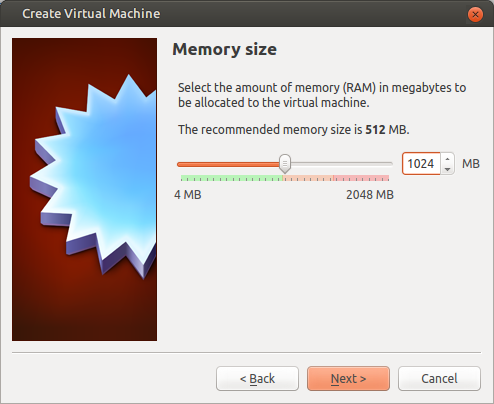
\includegraphics[width=\linewidth]{images/virtualbox_wizard2.png}
\end{wrapfigure}

W tym miejscu ustaw ilość pamięci operacyjnej twojego komputera, jaką chcesz przeznaczyć dla systemu-gościa. Weź pod uwagę, że ta pamięć zostanie zajęta w momencie uruchomienia maszyny wirtualnej i nie będzie dostępna dla systemu-gospodarza. Nie powinno się przydzielać gościowi więcej niż 50\% zasobów gospodarza. Ubuntu wymaga minimum 512 megabajtów (system plus oprogramowanie), a zdecydowanie lepiej jest przydzielić 1024 megabajty. Jeżeli twój komputer posiada tylko 2 gigabajty RAM-u, to przydzielając 1~gigabajt gościowi pozostanie tylko 1 gigabajt dla gospodarza. Nie jest to dobre rozwiązanie, gdyż prawdopodobnie będziesz musiał wyłączyć większość programów w systemie-gospodarzu, aby nie doszło do przepełnienia pamięci operacyjnej. Na pewno będziesz musiał wyłączyć przeglądarkę internetową.

\begin{flushright}
Kliknij przycisk \textcolor{ubuntu_orange}{Next}, aby przejść dalej.
\end{flushright}

W kolejnym oknie można wybrać już istniejący wirtualny dysk twardy lub stworzyć nowy. Ponieważ nie masz jeszcze żadnego takiego urządzenia, wybierz środkową opcję \textcolor{ubuntu_orange}{Create a virtual hard drive now}.
\begin{flushright}
Kliknij przycisk \textcolor{ubuntu_orange}{Next}, aby przejść dalej.
\end{flushright}

W kolejnym oknie wybierz typ dysku twardego. Zaznacz opcję \textcolor{ubuntu_orange}{VDI (Virtual Disk Image)}.
\begin{flushright}
Kliknij przycisk \textcolor{ubuntu_orange}{Next}, aby przejść dalej.
\end{flushright}

W kolejnym oknie wybierz pomiędzy dyskiem tworzonym dynamicznie, a dyskiem o stałym rozmiarze.
\begin{itemize}
\item \textcolor{ubuntu_orange}{Dynamically allocated} --- taki wirtualny dysk twardy nie zajmuje całego przydzielonego miejsca, a jedynie tyle, ile wynosi suma rozmiaru plików na nim zapisanych. Nawet jeżeli stworzysz dysk o pojemności 100 gigabajtów, to po instalacji Ubuntu będzie on zajmował tylko trochę ponad 6 gigabajtów w systemie-gospodarzu. Wybierz tę opcję.
\item \textcolor{ubuntu_orange}{Fixed size} --- taki dysk twardy zawsze zajmuje tyle miejsca w systemie-gospodarzu, ile zostało zadeklarowane. Jeżeli stworzysz 100-gigabajtowy dysk wirtualny, to na twoim komputerze pojawi się 100-gigabajtowy plik z maszyną wirtualną. Tworzenie takiego dysku też trwa dłuższą chwilę, gdyż dużo danych musi zostać zapisanych na dysk.
\end{itemize}
\begin{flushright}
Kliknij przycisk \textcolor{ubuntu_orange}{Next}, aby przejść dalej.
\end{flushright}
\clearpage
\begin{wrapfigure}[12]{r}{0.5\textwidth}
	\vspace{-10pt}
	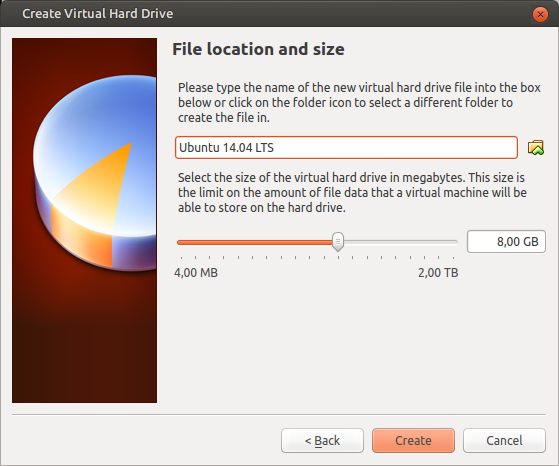
\includegraphics[width=\linewidth]{images/virtualbox_wizard6.png}
\end{wrapfigure}

Tu możesz wybrać pojemność dysku twardego. Korzystając z suwaka ustaw żądany rozmiar. Ubuntu 14.04 LTS wymaga przynajmniej 6,2 gigabajta, górną granicą są tylko możliwości VirtualBoksa (2 terabajty). W celach testowych stwórz dysk o rozmiarze przynajmniej 25 gigabajtów.

Kliknij przycisk \textcolor{ubuntu_orange}{Create}, aby stworzyć dysk i zakończyć działanie kreatora.

Twoja maszyna wirtualna dla Ubuntu jest gotowa i można ją wybrać w głównym oknie programu VirtualBox. Kliknij na jej nazwie i z paska narzędziowego wybierz \textcolor{ubuntu_orange}{Start}. Alternatywnym sposobem uruchomienia maszyny wirtualnej jest dwukrotne kliknięcie na jej ikonie. Zobaczysz okno, jak na rysunku powyżej. Kliknij żółtą ikonę folderu i wskaż pobrany wcześniej obraz instalatora systemu Ubuntu (plik .iso). Kliknij \textcolor{ubuntu_orange}{Start}, aby uruchomić maszynę wirtualną. Instalacja na maszynie wirtualnej przebiega tak samo, jak w rzeczywistości. Przejdź do sekcji \ref{instalacja_uruchomienie}: ,,Uruchomienie instalatora BIOS''.

\begin{center}
	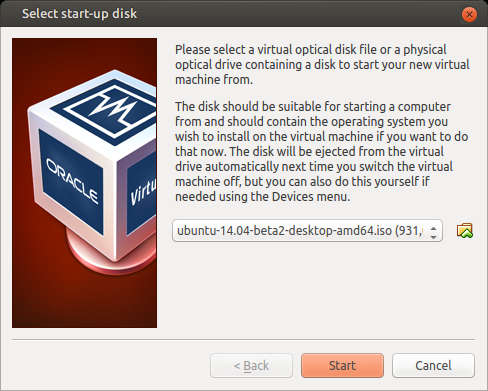
\includegraphics[width=\linewidth]{images/virtualbox_start.png}
\end{center}

Kiedy po zakończeniu instalacji zostaniesz poproszony o wyjęcie płyty instalatora z napędu, z paska menu maszyny wirtualnej wybierz \menu{{Devices}>{Cd/DVD Devices}>{Remove disk from virtual drive}}.

Żeby móc się cieszyć pełnosprawną maszyną wirtualną, należy doinstalować w systemie-gościu \textcolor{ubuntu_orange}{Używanie x86 virtualization solution --- guest addition module source for dkms z virtualbox-guest-dkms (własnościowy)}, zgodnie z instrukcją zawartą w \ref{pierwsze_uruchomienie_aktualizacja_instalacja}: ,,Instalacja dodatkowych sterowników''.
